
\date{\today}
\documentclass[12pt]{article}
\usepackage{graphicx}
\usepackage[T1]{fontenc}


\begin{document}
\section{Przypadki użycia( Use Cases)}
\subsection{Diagram Stanów}
\begin{minipage}[H]{.45\textwidth}
\centering
    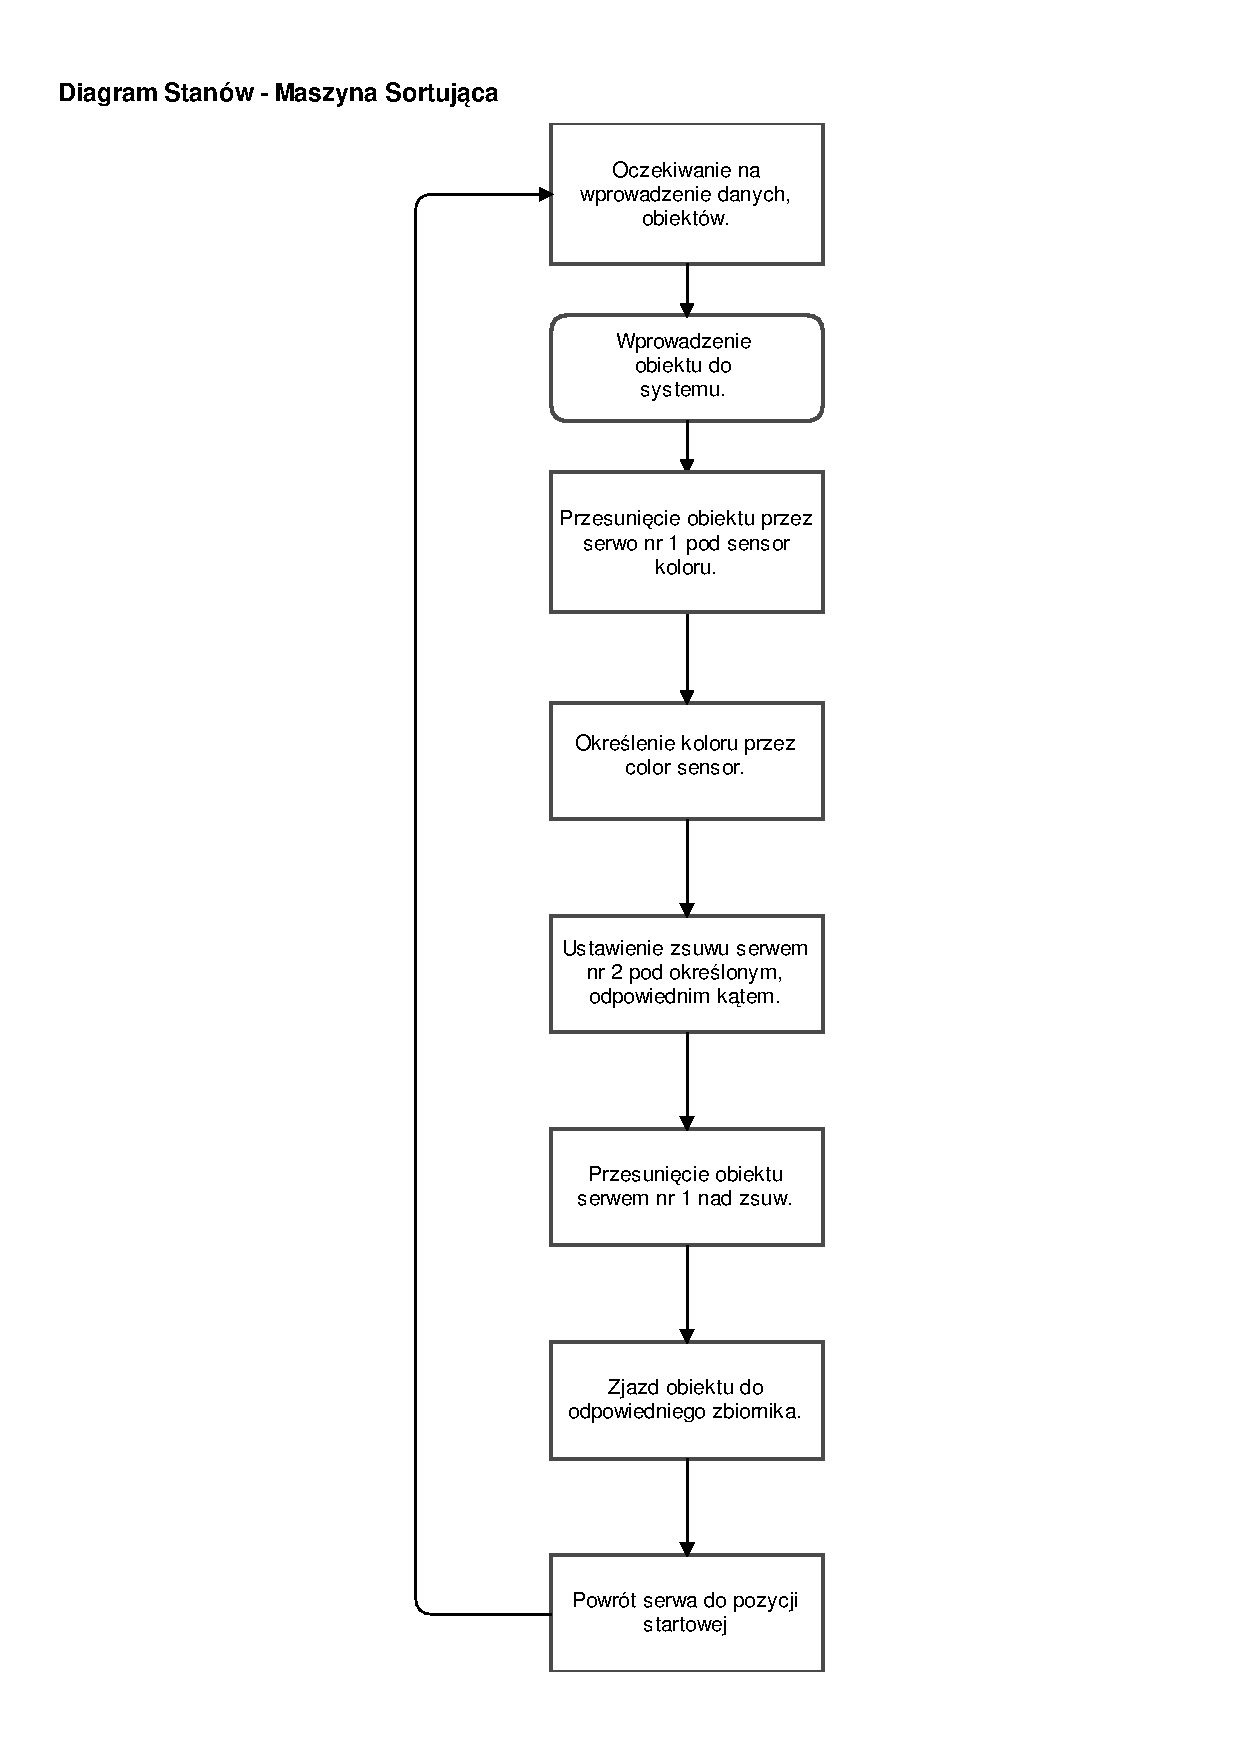
\includegraphics[height=2.8\linewidth]{diagram_stanow.pdf}
\end{minipage}
\subsection{Zasadniczy mechanizm realizowany przez system}
\subsubsection{Uruchomienie Systemu}
\paragraph{Przypadek Użycia:}\mbox{Nr 1}
\paragraph{Priorytet:}\mbox{Wysoki}	
\paragraph{Aktorzy:}\mbox{} \\
Operator uruchamia system, uzyskuje możliwość pracy na urządzeniu.\\
System uzyskuje dostęp do energii( zasilania), dzięki czemu może wykonywać działania.
\paragraph{Opis:}\mbox{} \\
System jest uruchamiany przez operatora dostępnym przyciskiem $ON/OFF.$

\subsubsection{Wprowadzenie Danych}
\paragraph{Przypadek Użycia:}\mbox{Nr 2}
\paragraph{Priorytet:}\mbox{Wysoki}	
\paragraph{Aktorzy:}\mbox{} \\
Operator wprowadza obiekt na wejście.\\
System otrzymuje dane niezbędne do rozpoczęcia działania.
\paragraph{Opis:}\mbox{} \\
Operator wprowadza obiekty do zbiornika, który będzie selekcjonowany. Jeden z obiektów wchodzi na główne wejście.

\subsubsection{Przekazanie obiektu do analizy}
\paragraph{Przypadek Użycia:}\mbox{Nr 3}
\paragraph{Priorytet:}\mbox{Wysoki}	
\paragraph{Aktorzy:}\mbox{} \\
System przenosi obiekt do miejsca, w którym zostanie on przeanalizowany.
\paragraph{Opis:}\mbox{} \\
System sam przekazuje przez serwo dane z wejścia pod sensor, gdzie zostanie przebadany.

\subsubsection{Analiza Obiektu}
\paragraph{Przypadek Użycia:}\mbox{Nr 4}
\paragraph{Priorytet:}\mbox{Wysoki}	
\paragraph{Aktorzy:}\mbox{} \\
System analizuje obiekt podany z wejścia. System otrzymuje informacje o obiekcie na podstawie, których może ustalić kolejne działania.
\paragraph{Opis:}\mbox{} \\
System analizuje obiekt w oparciu o sensor i określa jego kolor na podstawie określonych w implementacji zasad.

\subsubsection{Ustawienie Zsuwu}
\paragraph{Przypadek Użycia:}\mbox{Nr 5}
\paragraph{Priorytet:}\mbox{Wysoki}	
\paragraph{Aktorzy:}\mbox{} \\
System na podstawie posiadanych informacji ustawa zsuw w odpowiednim kącie.
\paragraph{Opis:}\mbox{} \\
System w zależności od uzyskanych danych ustala odpowiednią dla danych ścieżkę, po której ma zostać dalej przekazany obiekt do określonego miejsca.

\subsubsection{Zwolnienie obiektu}
\paragraph{Przypadek Użycia:}\mbox{Nr 6}
\paragraph{Priorytet:}\mbox{Wysoki}	
\paragraph{Aktorzy:}\mbox{} \\
System przenosi obiekt do zsuwu. 
Operator uzyskuje uporządkowany obiekt w oczekiwanym miejscu.
\paragraph{Opis:}\mbox{} \\
System przekazuje przez serwo obiekt nad poprawnie ustawiony zsuw, przy czym zwalnia obiekt do odpowiedniego kontenera. Po czym wraca do odpowiedniej pozycji oczekiwania na kolejny obiekt.






\end{document}